\documentclass[tcc]{subfiles}

\begin{document}
\textual

\subfile{text/body/introduction}

\chapter{Literature review}
\epigraph{To fight and conquer in all our battles is not supreme excellence; supreme excellence consists in breaking the enemy's resistance without fighting.}{\em(Sun Tzu)}

The simulation of a gas turbine engine is fundamentally a multidisciplinary matter.
It encompass not only the fields of turbomachinery and compressible flow, 
but also those of dynamical systems and numerical analysis. 

\section{Basic compressible flow relations}
There are many consolidated references on compressible flow. 
This section will only list the relations essential to the development in \cref{sec:methods}. 
The reader should refer to \textcite{Anderson, Shapiro} for a more in depth discussion.

\section{Euler's equation}
\label{sec:euler_equation}
Euler's equation is a consequence of the application of the laws of conservation of angular momentum and energy to a turbomachine. It is the cornerstone of performance calculation for compressor and turbines, and is derived in any textbook on turbomachinery \cite{Lakshminarayana1996, Dixon1998, Schobeiri2004, Hill1991, Logan2003, Baskharone2006}. Due to its importance, this equation will be briefly derived here.

From the conservation of angular momentum, 

\begin{equation}
    \vec{\acs{torque}} = \dot{m} (\vec{r}_{\text{out}}\cross\vec{V}_{\text{out}} - \vec{r}_{\text{in}}\cross\vec{V}_{\text{in}}) 
\end{equation}

Multiplying both sides by the rotational speed ($\omega$)

\begin{equation}
    \acs{power} = \vec{\omega}\cdot\vec{\acs{torque}} 
                = \dot{m} \vec{\omega} \cdot (\vec{r}_{\text{out}}\cross\vec{V}_{\text{out}} - \vec{r_{\text{in}}}\cross\vec{V}_{\text{in}}) 
\end{equation}

Assuming that the system is adiabatic and using the first law of thermodynamics, the specific enthalpy change is given by

\begin{equation}
    \Delta h = \frac{\acs{power}}{\dot{m}} 
             = \vec{\omega} \cdot (\vec{r}_{\text{out}}\cross\vec{V}_{\text{out}} - \vec{r}_{\text{in}}\cross\vec{V}_{\text{in}}) 
\end{equation}

\begin{equation}
    \Delta h = \omega (r_{\text{out}} {V_u}_{\text{out}} - r_{\text{in}} {V_u}_{\text{in}}) 
\end{equation}

\begin{equation}
    \label{eqn:euler}
    \Delta h = U_{\text{out}} {V_u}_{\text{out}} - U_{\text{in}} {V_u}_{\text{in}} 
\end{equation}

\subsection{Euler's equation for a centrifugal compressor}

It is useful to write the absolute tangential velocity at the compressor exit (${V_u}_3$)
as a function of the radial relative velocity (${W_r}_3$),
since the latter is more closely related to the mass flow 
(i.e. $\dot{m} = \rho {W_r}_3 A_3$, where $A_3$ is the ring shaped exit area of the compressor)

From the velocity triangle in figure X, assuming that the flow exits tangential to the blade surface,
\begin{equation}
    \label{eqn:V_u_3}
    {V_u}_3 = U_3 - {W_r}_3 \tan\beta_3
\end{equation}

Due to aerodynamic blockage at the tip and flow distortions caused by viscous efects, flow diffusion, clearences and blade aspect ratio,
${V_u}_3$ is actually smaller than what is predicted by \cref{eqn:V_u_3}.
This is accounted for by the \acf{impeller_distortion_factor}\index{impeller distortion factor}.
Furthermore, the flow does not exit perfectly tangential to the blade surface, and this is accounted by the \acf{slip_factor} \cite{Wiesner1967,Aungier1995}.
The corrected equation for the absolute tangential velocity is then

\begin{equation}
    \label{eqn:V_u_3_corrected}
    {V_u}_3 = \acs{slip_factor}(U_3 - \acs{impeller_distortion_factor}{W_r}_3 \tan\beta_3)
\end{equation}

Substituting \cref{eqn:V_u_3_corrected} in \cref{eqn:euler} and dividing both sides by ${U_3^2}$, we have

\begin{equation}
    \acs{load_coef}_c = \acs{slip_factor}(1-\acs{impeller_distortion_factor}\acs{flow_coef}_3\tan\beta_3) - \frac{U_2 {V_u}_2}{U_3^2} 
\end{equation}

where $\phi_3 \triangleq \frac{\dot{m}}{A_3 \rho_3 U_3} = \frac{W_{3r}}{U_3}$ is the flow parameter\index{flow parameter} at the compressor exit
and $\psi_c \triangleq \frac{\Delta h}{U_3^2}$ is the compressor power coefficient.

The second term accounts for pre-whirl\index{pre-whirl} in the flow entering the compressor, e.g due to \ac{IGV}.
In the case of no pre-whirl, ${V_u}_2 = 0$, thus 

\begin{equation}
    \label{eqn:euler}
    \boxed{\acs{load_coef}_c = \acs{slip_factor}(1-\acs{impeller_distortion_factor}\acs{flow_coef}_3\tan\beta_3)}
\end{equation}

\subsection{Euler's equation for an axial turbine}
\begin{figure}
    \centering
    \caption{Velocity triangle for an axial turbine stage}
%    \includegraphics[width=10cm]{fig/turbine_euler}
    \label{fig:turbine_euler}
    \source{\cite{Mattingly1996}}
\end{figure}

Applying \cref{eqn:euler} to an axial turbine stage (\cref{fig:turbine_euler}), we have
\begin{equation}
    \Delta_h = U_5V_5-U_4V_5
\end{equation}
The tangential fluid velocities can be expressed in terms of their axial components, i.e.\
\begin{align}
    V_{4u} &= V_{4x} \tan\alpha_4 \\
    V_{5u} &= U_5 + V_{5x} \tan\beta_5
\end{align}
Then,
\begin{equation}
    \Delta h = U_5^2 + U_5 V_{5x}\tan\beta_5 - U_4 V_{4x}\tan\alpha_4
\end{equation}
And finally, making the equation non-dimensional by diving both sides by the blade speed at the exit $U_5$, we get
\begin{equation}
    \boxed{\psi_t = 1 + \phi_5\tan\beta_5-\left(\frac{r_4}{r_5}\right)^2\phi_4\tan\alpha_4}
\end{equation}
where $\phi_4 = \frac{V_{4x}}{U_5}$ and $\phi_5 = \frac{V_{5x}}{U_5}$ are the flow parameters and
$\psi_t=\frac{\Delta h}{U_5^2}$ is the power coefficient for the turbine.

\section{Loss models for centrifugal compressors}
\label{sec:compressor_losses}
Euler's equation is only valid for isentropic flow. 
For a real flow, corrections must be introduced to account for the generation of entropy in many parts of the compression process. 
These so called ``losses'' are modelled in literature as enthalpy corrections 
for the Euler equation considering both the \emph{actual} process and the \emph{isentropic} process 
that would generate the same increase in pressure as the real process.
Each of these losses can be categorized as either \emph{internal} or \emph{parasitic}.
Internal losses are those that happen inside the fluid main flow, and result in a decrease in the resulting pressure ratio.
Parasitic losses are the ones who happen outside the fluid main flow, 
and result in a increase in the temperature ratio through the compressor \cite{Galvas1973}.
Using these definitions, the actual and isentropic enthalpy changes through the compressor can be calculate as follows

\begin{align}
    \Delta h_{\text{actual}} &= \Delta h_{\text{euler}} + \sum_{\substack{
                                                            \text{parasitic} \\ 
                                                            \text{losses}
                                                        }}
                                                          \Delta h \\
    \Delta h_{\text{isen}}  &= \Delta h_{\text{euler}} - \sum_{\substack{
                                                            \text{internal} \\ 
                                                            \text{losses}
                                                        }}
                                                          \Delta h
\end{align}

The temperature and pressure ratios are given by
\begin{align}
    \frac{T_{03}}{T_{02}} &= 1 + \frac{\Delta h_{\text{actual}}}{c_p T_{02}} \\
    \frac{P_{03}}{P_{02}} &= \left( 1 + \frac{\Delta h_{\text{isen}}}{c_p T_{02}}\right)^{\frac{\gamma}{\gamma-1}}
\end{align}

The isentropic and polytropic efficiencies can then be readly calculated as
\begin{align}
    \eta_t &= \frac{\Delta h_{\text{isen}}}{\Delta h_{\text{actual}}}\\
    \eta_p &= \frac{\gamma-1}{\gamma} \left(\frac{\log\frac{P_{02}}{P_{01}}}
                                                 {\log\frac{T_{02}}{T_{01}}}
                                     \right)
\end{align}

\textcite{Aungier1995} criticises this calculation because the losses should be regarded as changes in entropy, and not in enthalphy. Despite this shortcomming, the enthalphy approach is widely used.

The losses generally accounted for are listed in \cref{tbl:compressor_loss_mechanisms}. According to \textcite{Gravdahl2004,Gravdahl1999,Ferguson1963,Watson1982}, the most important losses for stability considerations are the incidence losses and the skin friction losses. The former is destabilizing because it introduces the positive slope of the left hand side of the compressor map. The fluid friction losses are stabilizing because they increase with mass flow, therefore contributing to the decrease in the derivative of the iso-speed lines.
\begin{table}
\caption{Loss mechanisms for a centrifugal compressor}
\label{tbl:compressor_loss_mechanisms}
\hrule
\begin{multicols}{2}
\begin{compactitem}
    \item[] \textbf{Internal}
    \item Incidence loss (in the impeller and diffuser)
    \item Blade loading loss
    \item Skin friction loss
    \item Clearance loss
    \item Mixing loss
    \item Vaneless diffuser loss
    \columnbreak
    \item[] \textbf{Parasitic}
    \item Disc friction loss
    \item Recirculation loss
    \item Leakage loss
\end{compactitem}
\end{multicols}
\hrule
\source{\cite{Oh1997}}
\end{table}

A detailed discussion of each loss mechanism is beyond the scope of this work; 
the interested reader should refer to \textcite{Cumpsty2004}. 

Semi-empirical models are available to predict each individual loss based on compressor geometry and flow conditions. 
In particular, \textcite{Oh1997} did a review of various loss models for each loss mechanism and selected an optimal set.

\section{Loss models for axial turbines}
Carter's rule
Ainsley

\section{Engine simulation (dynamic and static)}

The engine model used is of the lumped volume type. This means that each component 
 (compressor, combustor,turbine and nozzle)
 is modelled as a single point in space and conservation laws are applied to them.
 This type of model is also known as zero dimensional (0-D) or as parametric cycle analysis
 \index{parametric cycle analysis},
 and is widely used in both industry and academy as a tool for preliminary design and 
 performance analysis. 

A schematic of the engine components considered for the simulation of the present gas turbine engine is shown in \todo{add figure}.

\subsection{Turbojet thermodynamic cycle}

The thermodynamic cycle of gas turbines is the subject of many books \cite{Mattingly1996, Cumpsty2015}, 
and will only be discussed here in brief.

\subsection{What is a component map/characteristic}


\subsection{Available programs}

There are many readily available computer programs that implement this kind of simulation. 
From these, the most famous is probably the commercial program GasTurb \cite{GasTurb}, 
\index{software} \index{GasTurb}
followed by the \gls{GSP} \cite{Visser2000}.
A comparison of both is presented in \textcite{GasTurbvsGSP}.
In particular, GasTurb has already been used to simulate model gas turbines 
\cite{gao2011modelling}.
An open-source alternative is the \gls{T-MATS}, from NASA \cite{T-MATS}.
\gls{T-MATS} provides a library of turbo machinery blocks for use in Simulink. 
Each of these blocks is actually a wrapper for a function written in C 
that simulates the component's behaviour.

\section{Flow stability: compressor surge}
\section{Numerical aspects}
\subsection{Nonlinear solvers}
\subsubsection{Gradient based solvers}
\subsubsection{Homotopic solvers}
\subsection{\ac{ODE} solvers}
\subsubsection{Explicit solvers}
\subsubsection{Implicit solvers}
\subsection{Graph theory}
\subsubsection{Viewing a grid/mesh as a graph}
\subsubsection{Breadth first search}

\chapter{Methods}
\label{sec:methods}
\epigraph{It's not denial. \\ I'm just selective about the reality I accept.}{Bill Watterson}
Assumptions: ideal gas
\section{Compressor model}

The incidence loss model used assumes that all kinectic energy from the velocity components
normal to the inducer and diffuser blades is lost \cite{Stanitz1953}.
All other loss models used were suggested by the comparative study of \textcite{Oh1997}, 
and will not be discussed here.

\subfile{text/body/compressor_map}

From the Buckinham $\Pi$ Theorem \cite{Buckingham1914}, 
it can be shown that the compressor behaviour is a function of only three parameters, 
namely the \acl{MFP}, the \acl{M0rotor}, the \acl{gam} and the \acl{Re}. 
For a centrifugal compressor, this quantities are defined respectively as follows

\begin{align}
    \acs{MFP} &\triangleq \MFP{1} = \MFPalt{1} \\
    \acs{M0rotor} &\triangleq \frac{U_3}{\sqrt{\gamma R T_{01}}} \\
    \gamma &\triangleq \frac{c_p}{c_v} \\
    \acs{Re} &
\end{align}

In particular, the \acl{MFP} is a function of the Mach number and the specific heat ratio,
 i.e.\
\begin{equation}
    \label{eqn:mfp2mach}
    \acs{MFP}(M,\gamma) = M \left( 1 + \frac{\gamma-1}{2}M^2\right)^{-\frac{\gamma+1}{2(\gamma-1)}}
\end{equation}
While there is no closed form inverse for this function, it is invertible and the inverse can be easily computed nummerically, e.g.\ by a newton scheme \cite{Der1974}.

According to \textcite{walsh2004gas},
 the influence of the \acl{Re} in the system behaviour is only of second order.

To write Euler's equation \cref{eqn:euler} in terms of these parameters, suffices to rewrite $\phi_3$ and $\psi$ as a function of them. Thus
\begin{multline}
    \label{eqn:phi2_dimensionless}
    \phi_3 = \frac{W_{2r}}{U_3} 
           = \frac{\frac{\dot{m}}{\rho_3 A2}}{\acs{M0rotor} a_{02}}
           = \frac{\MFPalt{2}}{\acs{M0rotor}} \frac{a_{03}}{a_{02}} \stagdensratio{3} \\ 
           = \frac{\acs{MFP}_3}{\acs{M0rotor}} \sqrt{\frac{T_{03}}{T_{01}}} \stagdensratio{3}
\end{multline}
The value of $M_3$ can be obtained from $\acs{MFP}_3$ using \cref{eqn:mfp2mach}, while the latter is given by
\begin{equation}
    \label{eqn:mfp2mfp2}
    \acs{MFP}_3 \triangleq \MFP{2} = \acs{MFP} \frac{A_2}{A_3} \frac{P_{02}}{P_{03}} \sqrt{\frac{T_{03}}{T_{02}}}
\end{equation}
Notice that \cref{eqn:mfp2mfp2} makes no assumption of the process 1--2 being isentropic. $\acs{MFP}_3$ can be used along with \acs{MFP} to check for choking.

The load coefficient is given by
\begin{equation}
    \acs{load_coef}\triangleq \frac{\Delta h}{U_3^2}
                      = \frac{c_p(T_{02}-T_{02})}{U_3^2}
                      = \frac{\frac{c_p(T_{03}-T_{01})}{\gamma R T_{02}}}
                                    {\acs{M0rotor}^2}
                      = \frac{\frac{T_{03}}{T_{02}}-1}
                                  {\acs{M0rotor}^2}
                        \left(\frac{1}{\gamma-1}\right)
\end{equation}

At this point the loss models discussed in \cref{sec:compressor_losses} are introduced, 
and the values of $\acs{load_coef}_{\text{actual}}$ and $\acs{load_coef}_{\text{isen}}$ are obtained.
The temperatures and pressure ratio can then be readly calculate from
\begin{align}
    \label{eqn:psi2Tratio}
    \frac{T_{03}}{T_{02}} &= (\gamma - 1)\psi_{\text{actual}} \acs{M0rotor}^2 + 1 \\
    \label{eqn:psi2Pratio}
    \frac{P_{03}}{P_{02}} &= \left[(\gamma - 1)\psi_{\text{isen}} \acs{M0rotor}^2 + 1\right]^\frac{\gamma}{\gamma-1}
\end{align}


\section{Turbine model}
\subfile{text/body/turbine_map}

\subfile{text/body/nozzle}


\section{Engine equilibrium model}


The engine equilibrium, or steady state, 


Equations:
\begin{enumerate}
    \item Constant shaft speed
    \item Conservation of mass in the burner
    \item Energy adition due to fuel
    \item nozzle
    \item turbine (x3)
    \item compressor (x3)
\end{enumerate}

\section{Engine dynamical model}
\begin{align}
    \dot{P}_{04} &= \frac{a_{01}^2}{\volume}(\dot{m}_c - \dot{m}_t) \\
    \ddot{m}_c &= \frac{A_1}{L_c}(P_{03}-P_{04}) \\
    \dot{\omega} &= \frac{1}{J} (\tau_t-\tau_c)
\end{align}

\section{Surge model}
\section{Numerical aspects}
\subsection{Nonlinear solvers and convergence}
\subsection{Generating a parametric surface from a nonlinear system}
\subsubsection{Initial guess propagation}

\chapter{Results and discussion}
\epigraph{``Que tanto de coisa para estragar.''\\{\footnotesize ``That's a lot of parts to need fixing.}''}{My Grandfather commenting on my dad's new car}
\section{Compressor map}
\section{Turbine map}
\section{Work line}

\begin{sidewaysfigure}[p]
    \AddThispageHook{\thispagestyle{empty}}
    \caption{Component maps and work line of the VT-80 engine}
\includegraphics{fig/wline.pdf}
    \source{author's figure}
    \legend{Compressor and turbine maps for the VT-80 engine, with the work line superimposed (thick line).
    The medium thickness contours are of constant blade mach number and the thin countours are of constant polytropic efficiency.}
\end{sidewaysfigure}

\section{Dynamical simulation}
\subfile{text/body/materials_and_methods}
\subfile{text/body/dynamic_engine_model}
\subfile{text/body/controller_model}
\subfile{text/body/conclusion}

\end{document}
